\section{红黑树}

\subsection{红黑树(Red Black Tree)}

红黑树是一种自平衡的二叉查找树,除了符合二叉查找树的基本特性外,它还具有如下附加特性:

\begin{enumerate}
    \item 结点是红色或黑色的。
    \item 根结点是黑色的。
    \item 叶子结点都是黑色的空结点NIL。
    \item 红色结点的两个子结点都是黑色的,即从叶子到根的所有路径上不能有连续的两个红色结点。
    \item 从任一结点到其每个叶子的所有路径都包含相同数目的黑色结点。
\end{enumerate}

\begin{figure}[H]
    \centering
    \begin{tikzpicture}[font=\sffamily, very thick,
            level distance=1.5cm,
            level 1/.style={sibling distance=8cm},
            level 2/.style={sibling distance=4cm},
            level 3/.style={sibling distance=2cm},
            level 4/.style={sibling distance=1cm},
        ]
        \node [blackVertex] (r){13}
        child {
                node [redVertex] {8}
                child {
                        node [blackVertex] {1}
                        child {node [nil] {NIL}}
                        child {
                                node [redVertex] {6}
                                child {node [nil] {NIL}}
                                child {node [nil] {NIL}}
                            }
                    }
                child {
                        node [blackVertex] {11}
                        child {node [nil] {NIL}}
                        child {node [nil] {NIL}}
                    }
            }
        child {
                node [redVertex] {17}
                child {
                        node [blackVertex] {15}
                        child {node [nil] {NIL}}
                        child {node [nil] {NIL}}
                    }
                child {
                        node [blackVertex] {25}
                        child {
                                node [redVertex] {22}
                                child {node [nil] {NIL}}
                                child {node [nil] {NIL}}
                            }
                        child {
                                node [redVertex] {27}
                                child {node [nil] {NIL}}
                                child {node [nil] {NIL}}
                            }
                    }
            };
    \end{tikzpicture}
    \caption{红黑树}
\end{figure}

天呐,这条条框框的太多了吧! \\

正是因为这些规则限制,才保证了红黑树的自平衡,红黑树从根到叶子的最长路径不会超过最短路径的2倍。 \\

红黑树的应用有很多,其中JDK的集合类TreeMap和TreeSet底层就是红黑树实现的。在Java8中,连HashMap也用到了红黑树。

\subsection{失衡调整}

当插入或删除结点时,红黑树的规则可能被破坏,需要调整使其重新符合规则。 \\

例如向红黑树中插入新结点14,由于父结点15是黑色结点,这种情况不会破坏红黑树的规则,无需做任何调整。

\begin{figure}[H]
    \centering
    \begin{tikzpicture}[font=\sffamily, very thick,
            level distance=1.5cm,
            level 1/.style={sibling distance=8cm},
            level 2/.style={sibling distance=4cm},
            level 3/.style={sibling distance=2cm},
            level 4/.style={sibling distance=1cm},
        ]
        \node [blackVertex] (r){13}
        child {
                node [redVertex] {8}
                child {
                        node [blackVertex] {1}
                        child {node [nil] {NIL}}
                        child {
                                node [redVertex] {6}
                                child {node [nil] {NIL}}
                                child {node [nil] {NIL}}
                            }
                    }
                child {
                        node [blackVertex] {11}
                        child {node [nil] {NIL}}
                        child {node [nil] {NIL}}
                    }
            }
        child {
                node [redVertex] {17}
                child {
                        node [blackVertex] {15}
                        child {
                                node [redVertex] {14}
                                child {node [nil] {NIL}}
                                child {node [nil] {NIL}}
                            }
                        child {node [nil] {NIL}}
                    }
                child {
                        node [blackVertex] {25}
                        child {
                                node [redVertex] {22}
                                child {node [nil] {NIL}}
                                child {node [nil] {NIL}}
                            }
                        child {
                                node [redVertex] {27}
                                child {node [nil] {NIL}}
                                child {node [nil] {NIL}}
                            }
                    }
            };
    \end{tikzpicture}
    \caption{插入14}
\end{figure}

向红黑树中插入新结点21,由于父结点22是红色结点,违反了红黑树的规则4(红色结点的两个子结点都是黑色的)。

\begin{figure}[H]
    \centering
    \begin{tikzpicture}[font=\sffamily, very thick,
            level distance=1.5cm,
            level 1/.style={sibling distance=8cm},
            level 2/.style={sibling distance=4cm},
            level 3/.style={sibling distance=2cm},
            level 4/.style={sibling distance=1cm},
        ]
        \node [blackVertex] (r){13}
        child {
                node [redVertex] {8}
                child {
                        node [blackVertex] {1}
                        child {node [nil] {NIL}}
                        child {
                                node [redVertex] {6}
                                child {node [nil] {NIL}}
                                child {node [nil] {NIL}}
                            }
                    }
                child {
                        node [blackVertex] {11}
                        child {node [nil] {NIL}}
                        child {node [nil] {NIL}}
                    }
            }
        child {
                node [redVertex] {17}
                child {
                        node [blackVertex] {15}
                        child {node [nil] {NIL}}
                        child {node [nil] {NIL}}
                    }
                child {
                        node [blackVertex] {25}
                        child {
                                node [redVertex] {22}
                                child {
                                        node [redVertex] {21}
                                        child {node [nil] {NIL}}
                                        child {node [nil] {NIL}}
                                    }
                                child {node [nil] {NIL}}
                            }
                        child {
                                node [redVertex] {27}
                                child {node [nil] {NIL}}
                                child {node [nil] {NIL}}
                            }
                    }
            };
    \end{tikzpicture}
    \caption{插入21}
\end{figure}

调整的方法有变色和旋转两种,而旋转又包含左旋转和右旋转两种方式。 \\

为了重新符合红黑树的规则,有时需要把红色结点变为黑色,或是把黑色结点变为红色。 \\

例如对于红黑树的一部分(子树),新插入的结点Y是红色结点,它的父结点X也是红色结点,不符合规则4(红色结点的两个子结点都是黑色的),因此可以把结点X变为黑色。

\begin{figure}[H]
    \centering
    \begin{tikzpicture}[font=\sffamily, very thick,
            level distance=1.5cm,
            level 1/.style={sibling distance=4cm},
            level 2/.style={sibling distance=2cm},
            level 3/.style={sibling distance=1cm}
        ]
        \node [redVertex] (r){X}
        child {
                node [redVertex] {Y}
                child {node [nil] {NIL}}
                child {node [nil] {NIL}}
            }
        child {node [nil] {NIL}};
    \end{tikzpicture}
    \caption{违反规则4}
\end{figure}

\begin{figure}[H]
    \centering
    \begin{tikzpicture}[font=\sffamily, very thick,
            level distance=1.5cm,
            level 1/.style={sibling distance=4cm},
            level 2/.style={sibling distance=2cm},
            level 3/.style={sibling distance=1cm}
        ]
        \node [blackVertex] (r){X}
        child {
                node [redVertex] {Y}
                child {node [nil] {NIL}}
                child {node [nil] {NIL}}
            }
        child {node [nil] {NIL}};
    \end{tikzpicture}
    \caption{变色}
\end{figure}

但是,如果这是简单的把一个结点变色,会导致相关路径凭空多出一个黑色结点,这样就会打破规则5(从任一结点到其每个叶子的所有路径都包含相同数目的黑色结点),因此还需要其它的调整策略。

\subsection{红黑树插入结点}

红黑树插入新结点时,可以分为五种不同的局面。每一种局面有不同的调整方法。

\subsubsection{局面1}

新结点(A)位于树根,没有父结点。

\begin{figure}[H]
    \centering
    \begin{tikzpicture}[font=\sffamily, very thick,
            level distance=1.5cm,
            level 1/.style={sibling distance=2cm},
            level 2/.style={sibling distance=1cm}
        ]
        \node [redVertex] (r){A}
        child {node[rectangle,draw] {1}}
        child {node[rectangle,draw] {2}};
    \end{tikzpicture}
    \caption{局面1}
\end{figure}

这种局面,直接让新结点变色为黑色,规则2(根结点是黑色的)满足。同时黑色的根结点使每条路径上的黑色结点数目都增加了1,因此并没有打破规则5(从任一结点到其每个叶子的所有路径都包含相同数目的黑色结点)。

\begin{figure}[H]
    \centering
    \begin{tikzpicture}[font=\sffamily, very thick,
            level distance=1.5cm,
            level 1/.style={sibling distance=2cm},
            level 2/.style={sibling distance=1cm}
        ]
        \node [blackVertex] (r){A}
        child {node[rectangle,draw] {1}}
        child {node[rectangle,draw] {2}};
    \end{tikzpicture}
\end{figure}

\subsubsection{局面2}

新结点(B)的父结点是黑色的。新插入的红色结点B并没有打破规则,无需调整。

\begin{figure}[H]
    \centering
    \begin{tikzpicture}[font=\sffamily, very thick,
            level distance=1.5cm,
            level 1/.style={sibling distance=2cm},
            level 2/.style={sibling distance=1cm}
        ]
        \node [blackVertex] (r){A}
        child {
                node [redVertex] {B}
                child {node[rectangle,draw] {1}}
                child {node[rectangle,draw] {2}}
            }
        child {node[rectangle,draw] {3}};
    \end{tikzpicture}
    \caption{局面2}
\end{figure}

\subsubsection{局面3}

新结点(D)的父结点和叔叔结点都是红色。

\begin{figure}[H]
    \centering
    \begin{tikzpicture}[font=\sffamily, very thick,
            level distance=1.5cm,
            level 1/.style={sibling distance=2cm},
            level 2/.style={sibling distance=1cm},
            level 3/.style={sibling distance=1cm}
        ]
        \node [blackVertex] (r){A}
        child {
                node [redVertex] {B}
                child {
                        node [redVertex] {D}
                        child {node[rectangle,draw] {1}}
                        child {node[rectangle,draw] {2}}
                    }
                child {node[rectangle,draw] {3}}
            }
        child {
                node [redVertex] {C}
                child {node[rectangle,draw] {4}}
                child {node[rectangle,draw] {5}}
            };
    \end{tikzpicture}
    \caption{局面3}
\end{figure}

这种局面,两个红色结点B和D连续,违反了规则4(红色结点的两个子结点都是黑色的),因此需要先让结点B变为黑色。

\begin{figure}[H]
    \centering
    \begin{tikzpicture}[font=\sffamily, very thick,
            level distance=1.5cm,
            level 1/.style={sibling distance=2cm},
            level 2/.style={sibling distance=1cm},
            level 3/.style={sibling distance=1cm}
        ]
        \node [blackVertex] (r){A}
        child {
                node [blackVertex] {B}
                child {
                        node [redVertex] {D}
                        child {node[rectangle,draw] {1}}
                        child {node[rectangle,draw] {2}}
                    }
                child {node[rectangle,draw] {3}}
            }
        child {
                node [redVertex] {C}
                child {node[rectangle,draw] {4}}
                child {node[rectangle,draw] {5}}
            };
    \end{tikzpicture}
\end{figure}

但是这样一来,结点B所在路径凭空多出了一个黑色结点,打破了规则5(从任一结点到其每个叶子的所有路径都包含相同数目的黑色结点),因此再让结点A变为红色。

\begin{figure}[H]
    \centering
    \begin{tikzpicture}[font=\sffamily, very thick,
            level distance=1.5cm,
            level 1/.style={sibling distance=2cm},
            level 2/.style={sibling distance=1cm},
            level 3/.style={sibling distance=1cm}
        ]
        \node [redVertex] (r){A}
        child {
                node [blackVertex] {B}
                child {
                        node [redVertex] {D}
                        child {node[rectangle,draw] {1}}
                        child {node[rectangle,draw] {2}}
                    }
                child {node[rectangle,draw] {3}}
            }
        child {
                node [redVertex] {C}
                child {node[rectangle,draw] {4}}
                child {node[rectangle,draw] {5}}
            };
    \end{tikzpicture}
\end{figure}

这时结点A和C又成为了连续的红色结点,再将结点C变为黑色。

\begin{figure}[H]
    \centering
    \begin{tikzpicture}[font=\sffamily, very thick,
            level distance=1.5cm,
            level 1/.style={sibling distance=2cm},
            level 2/.style={sibling distance=1cm},
            level 3/.style={sibling distance=1cm}
        ]
        \node [redVertex] (r){A}
        child {
                node [blackVertex] {B}
                child {
                        node [redVertex] {D}
                        child {node[rectangle,draw] {1}}
                        child {node[rectangle,draw] {2}}
                    }
                child {node[rectangle,draw] {3}}
            }
        child {
                node [blackVertex] {C}
                child {node[rectangle,draw] {4}}
                child {node[rectangle,draw] {5}}
            };
    \end{tikzpicture}
\end{figure}

\subsubsection{局面4}

新结点(D)的父结点是红色,叔叔结点是黑色或者没有叔叔,且新结点是父结点的右孩子,父结点是祖父结点的左孩子。

\begin{figure}[H]
    \centering
    \begin{tikzpicture}[font=\sffamily, very thick,
            level distance=1.5cm,
            level 1/.style={sibling distance=2cm},
            level 2/.style={sibling distance=1cm},
            level 3/.style={sibling distance=1cm}
        ]
        \node [blackVertex] (r){A}
        child {
                node [redVertex] {B}
                child {node[rectangle,draw] {1}}
                child {
                        node [redVertex] {D}
                        child {node[rectangle,draw] {2}}
                        child {node[rectangle,draw] {3}}
                    }
            }
        child {
                node [blackVertex] {C}
                child {node[rectangle,draw] {4}}
                child {node[rectangle,draw] {5}}
            };
    \end{tikzpicture}
    \caption{局面4}
\end{figure}

这个局面可以以结点B为轴,做一次左旋转,使得新结点D成为父结点,结点B成为D的左孩子。这样一来进入了局面5。

\begin{figure}[H]
    \centering
    \begin{tikzpicture}[font=\sffamily, very thick,
            level distance=1.5cm,
            level 1/.style={sibling distance=2cm},
            level 2/.style={sibling distance=1cm},
            level 3/.style={sibling distance=1cm}
        ]
        \node [blackVertex] (r){A}
        child {
                node [redVertex] {D}
                child {
                        node [redVertex] {B}
                        child {node[rectangle,draw] {1}}
                        child {node[rectangle,draw] {2}}
                    }
                child {node[rectangle,draw] {3}}
            }
        child {
                node [blackVertex] {C}
                child {node[rectangle,draw] {4}}
                child {node[rectangle,draw] {5}}
            };
    \end{tikzpicture}
\end{figure}

\subsubsection{局面5}

新结点(D)的父结点是红色,叔叔结点是黑色或者没有叔叔,且新结点是父结点的左孩子,父结点是祖父结点的左孩子。

\begin{figure}[H]
    \centering
    \begin{tikzpicture}[font=\sffamily, very thick,
            level distance=1.5cm,
            level 1/.style={sibling distance=2cm},
            level 2/.style={sibling distance=1cm},
            level 3/.style={sibling distance=1cm}
        ]
        \node [blackVertex] (r){A}
        child {
                node [redVertex] {B}
                child {
                        node [redVertex] {D}
                        child {node[rectangle,draw] {1}}
                        child {node[rectangle,draw] {2}}
                    }
                child {node[rectangle,draw] {3}}
            }
        child {
                node [blackVertex] {C}
                child {node[rectangle,draw] {4}}
                child {node[rectangle,draw] {5}}
            };
    \end{tikzpicture}
    \caption{局面5}
\end{figure}

这一局面可以以结点A为轴,做一次右旋转,使得结点B成为祖父结点,结点A成为B的右孩子。

\begin{figure}[H]
    \centering
    \begin{tikzpicture}[font=\sffamily, very thick,
            level distance=1.5cm,
            level 1/.style={sibling distance=2cm},
            level 2/.style={sibling distance=1cm},
            level 3/.style={sibling distance=1cm}
        ]
        \node [redVertex] (r){B}
        child {
                node [redVertex] {D}
                child {node[rectangle,draw] {1}}
                child {node[rectangle,draw] {2}}
            }
        child {
                node [blackVertex] {A}
                child {node[rectangle,draw] {3}}
                child {
                        node [blackVertex] {C}
                        child {node[rectangle,draw] {4}}
                        child {node[rectangle,draw] {5}}
                    }
            };
    \end{tikzpicture}
\end{figure}

再将结点B变为黑色,结点A变为红色。

\begin{figure}[H]
    \centering
    \begin{tikzpicture}[font=\sffamily, very thick,
            level distance=1.5cm,
            level 1/.style={sibling distance=2cm},
            level 2/.style={sibling distance=1cm},
            level 3/.style={sibling distance=1cm}
        ]
        \node [blackVertex] (r){B}
        child {
                node [redVertex] {D}
                child {node[rectangle,draw] {1}}
                child {node[rectangle,draw] {2}}
            }
        child {
                node [redVertex] {A}
                child {node[rectangle,draw] {3}}
                child {
                        node [blackVertex] {C}
                        child {node[rectangle,draw] {4}}
                        child {node[rectangle,draw] {5}}
                    }
            };
    \end{tikzpicture}
\end{figure}

红黑树的插入操作设计到这5种局面。如果局面4中父结点B是右孩子,则成为了局面5的镜像,原本的右旋转改为左旋转;如果局面5中父结点B是右孩子,则成为了局面4的镜像,原本的左旋转改为右旋转。 \\

例如在一个红黑树中插入新结点21,需要根据不同局面进行调整。

\begin{figure}[H]
    \centering
    \begin{tikzpicture}[font=\sffamily, very thick,
            level distance=1.5cm,
            level 1/.style={sibling distance=8cm},
            level 2/.style={sibling distance=4cm},
            level 3/.style={sibling distance=2cm},
            level 4/.style={sibling distance=1cm},
        ]
        \node [blackVertex] (r){13}
        child {
                node [redVertex] {8}
                child {
                        node [blackVertex] {1}
                        child {node [nil] {NIL}}
                        child {node [nil] {NIL}}
                    }
                child {
                        node [blackVertex] {11}
                        child {node [nil] {NIL}}
                        child {node [nil] {NIL}}
                    }
            }
        child {
                node [redVertex] {17}
                child {
                        node [blackVertex] {15}
                        child {node [nil] {NIL}}
                        child {node [nil] {NIL}}
                    }
                child {
                        node [blackVertex] {25}
                        child {
                                node [redVertex] {22}
                                child {
                                        node [redVertex] {21}
                                        child {node [nil] {NIL}}
                                        child {node [nil] {NIL}}
                                    }
                                child {node [nil] {NIL}}
                            }
                        child {
                                node [redVertex] {27}
                                child {node [nil] {NIL}}
                                child {node [nil] {NIL}}
                            }
                    }
            };
    \end{tikzpicture}
\end{figure}

新结点21和它的父结点22是连续的红色结点,违背了规则4。当前情况符合局面3(新结点的父结点和叔叔结点都是红色)。于是经过三次变色(22变为黑色,25变为红色,27变为黑色),将以结点25为根的子树符合了红黑树的规则。

\begin{figure}[H]
    \centering
    \begin{tikzpicture}[font=\sffamily, very thick,
            level distance=1.5cm,
            level 1/.style={sibling distance=8cm},
            level 2/.style={sibling distance=4cm},
            level 3/.style={sibling distance=2cm},
            level 4/.style={sibling distance=1cm},
        ]
        \node [blackVertex] (r){13}
        child {
                node [redVertex] {8}
                child {
                        node [blackVertex] {1}
                        child {node [nil] {NIL}}
                        child {node [nil] {NIL}}
                    }
                child {
                        node [blackVertex] {11}
                        child {node [nil] {NIL}}
                        child {node [nil] {NIL}}
                    }
            }
        child {
                node [redVertex] {17}
                child {
                        node [blackVertex] {15}
                        child {node [nil] {NIL}}
                        child {node [nil] {NIL}}
                    }
                child {
                        node [redVertex] {25}
                        child {
                                node [blackVertex] {22}
                                child {
                                        node [redVertex] {21}
                                        child {node [nil] {NIL}}
                                        child {node [nil] {NIL}}
                                    }
                                child {node [nil] {NIL}}
                            }
                        child {
                                node [blackVertex] {27}
                                child {node [nil] {NIL}}
                                child {node [nil] {NIL}}
                            }
                    }
            };
    \end{tikzpicture}
\end{figure}

但结点25和结点17成为了连续的红色结点,违背了规则4。于是可以将结点25看做一个新结点,当前正好符合局面5的镜像(新结点的父结点是红色,叔叔是黑色或者没有叔叔,且新结点是父结点的右孩子,父结点是祖父结点的右孩子)。因此可以以根结点13为轴进行左旋转,使得结点17成为新的根结点。

\begin{figure}[H]
    \centering
    \begin{tikzpicture}[font=\sffamily, very thick,
            level distance=1.5cm,
            level 1/.style={sibling distance=8cm},
            level 2/.style={sibling distance=4cm},
            level 3/.style={sibling distance=2cm},
            level 4/.style={sibling distance=1cm},
        ]
        \node [redVertex] (r){17}
        child {
                node [blackVertex] {13}
                child {
                        node [blackVertex] {8}
                        child {
                                node [redVertex] {1}
                                child {node [nil] {NIL}}
                                child {node [nil] {NIL}}
                            }
                        child {
                                node [redVertex] {11}
                                child {node [nil] {NIL}}
                                child {node [nil] {NIL}}
                            }
                    }
                child {
                        node [blackVertex] {15}
                        child {node [nil] {NIL}}
                        child {node [nil] {NIL}}
                    }
            }
        child {
                node [redVertex] {25}
                child {
                        node [blackVertex] {22}
                        child {
                                node [redVertex] {21}
                                child {node [nil] {NIL}}
                                child {node [nil] {NIL}}
                            }
                        child {node [nil] {NIL}}
                    }
                child {
                        node [blackVertex] {27}
                        child {node [nil] {NIL}}
                        child {node [nil] {NIL}}
                    }
            };
    \end{tikzpicture}
\end{figure}

再让结点17变为黑色,13变为红色,使红黑树重新符合规则。

\begin{figure}[H]
    \centering
    \begin{tikzpicture}[font=\sffamily, very thick,
            level distance=1.5cm,
            level 1/.style={sibling distance=8cm},
            level 2/.style={sibling distance=4cm},
            level 3/.style={sibling distance=2cm},
            level 4/.style={sibling distance=1cm},
        ]
        \node [blackVertex] (r){17}
        child {
                node [redVertex] {13}
                child {
                        node [blackVertex] {8}
                        child {
                                node [redVertex] {1}
                                child {node [nil] {NIL}}
                                child {node [nil] {NIL}}
                            }
                        child {
                                node [redVertex] {11}
                                child {node [nil] {NIL}}
                                child {node [nil] {NIL}}
                            }
                    }
                child {
                        node [blackVertex] {15}
                        child {node [nil] {NIL}}
                        child {node [nil] {NIL}}
                    }
            }
        child {
                node [redVertex] {25}
                child {
                        node [blackVertex] {22}
                        child {
                                node [redVertex] {21}
                                child {node [nil] {NIL}}
                                child {node [nil] {NIL}}
                            }
                        child {node [nil] {NIL}}
                    }
                child {
                        node [blackVertex] {27}
                        child {node [nil] {NIL}}
                        child {node [nil] {NIL}}
                    }
            };
    \end{tikzpicture}
\end{figure}

\subsection{二叉查找树删除结点}

在介绍红黑树的删除操作之前,需要先理解二叉查找树的删除操作。 \\

二叉查找树的删除可分为三种情况:

\subsubsection{待删除结点无子结点}

如果待删除结点没有子结点,直接删除即可。

\begin{figure}[H]
    \centering
    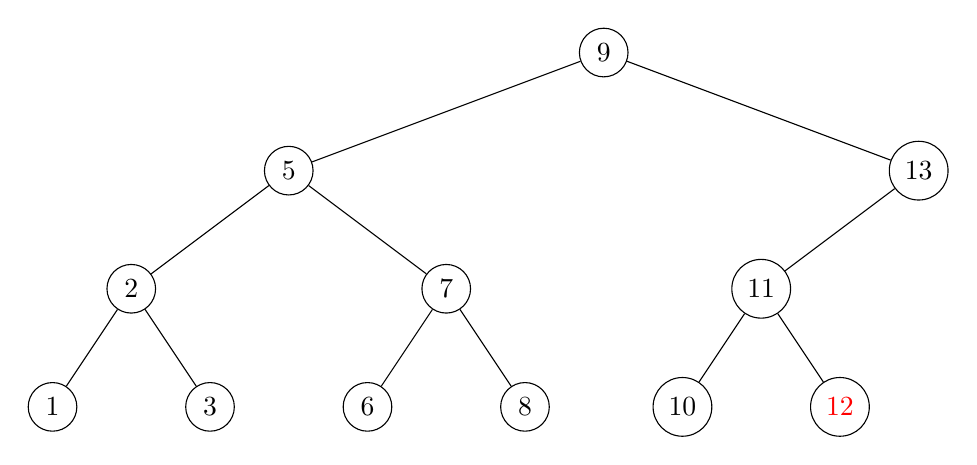
\begin{tikzpicture}[
            level distance=1.5cm,
            level 1/.style={sibling distance=8cm},
            level 2/.style={sibling distance=4cm},
            level 3/.style={sibling distance=2cm}
        ]
        \node[circle,draw] {9}
        child {
                node[circle,draw] {5}
                child {
                        node[circle,draw] {2}
                        child {node[circle,draw] {1}}
                        child {node[circle,draw] {3}}
                    }
                child {
                        node[circle,draw] {7}
                        child {node[circle,draw] {6}}
                        child {node[circle,draw] {8}}
                    }
            }
        child {
                node[circle,draw] {13}
                child {
                        node[circle,draw] {11}
                        child {node[circle,draw] {10}}
                        child {node[circle,draw] {\textcolor{red}{12}}}
                    }
                child[missing] {}
            };
    \end{tikzpicture}
    \caption{删除结点12}
\end{figure}

\subsubsection{待删除结点只有一个孩子}

如果待删除结点只有一个孩子,让孩子取代待被删除结点。

\begin{figure}[H]
    \centering
    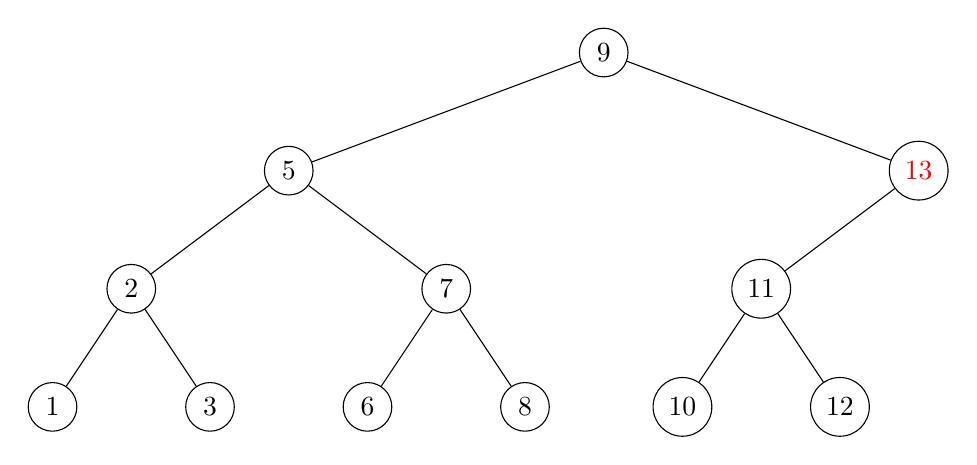
\begin{tikzpicture}[
            level distance=1.5cm,
            level 1/.style={sibling distance=8cm},
            level 2/.style={sibling distance=4cm},
            level 3/.style={sibling distance=2cm}
        ]
        \node[circle,draw] {9}
        child {
                node[circle,draw] {5}
                child {
                        node[circle,draw] {2}
                        child {node[circle,draw] {1}}
                        child {node[circle,draw] {3}}
                    }
                child {
                        node[circle,draw] {7}
                        child {node[circle,draw] {6}}
                        child {node[circle,draw] {8}}
                    }
            }
        child {
                node[circle,draw] {\textcolor{red}{13}}
                child {
                        node[circle,draw] {11}
                        child {node[circle,draw] {10}}
                        child {node[circle,draw] {12}}
                    }
                child[missing] {}
            };
    \end{tikzpicture}
    \caption{删除结点13}
\end{figure}

\begin{figure}[H]
    \centering
    \begin{tikzpicture}[
            level distance=1.5cm,
            level 1/.style={sibling distance=8cm},
            level 2/.style={sibling distance=4cm},
            level 3/.style={sibling distance=2cm}
        ]
        \node[circle,draw] {9}
        child {
                node[circle,draw] {5}
                child {
                        node[circle,draw] {2}
                        child {node[circle,draw] {1}}
                        child {node[circle,draw] {3}}
                    }
                child {
                        node[circle,draw] {7}
                        child {node[circle,draw] {6}}
                        child {node[circle,draw] {8}}
                    }
            }
        child {
                node[circle,draw] {11}
                child {node[circle,draw] {10}}
                child {node[circle,draw] {12}}
            };
    \end{tikzpicture}
\end{figure}

\subsubsection{待删除结点有两个孩子}

选择仅小于或仅大于待删除结点的结点取代,习惯上更多地会选择仅大于待删除结点的结点。

\begin{figure}[H]
    \centering
    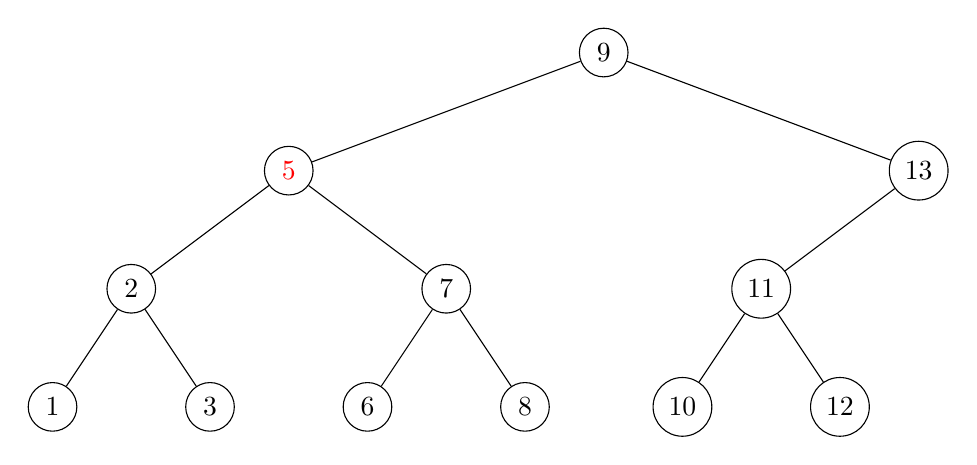
\begin{tikzpicture}[
            level distance=1.5cm,
            level 1/.style={sibling distance=8cm},
            level 2/.style={sibling distance=4cm},
            level 3/.style={sibling distance=2cm}
        ]
        \node[circle,draw] {9}
        child {
                node[circle,draw] {\textcolor{red}{5}}
                child {
                        node[circle,draw] {2}
                        child {node[circle,draw] {1}}
                        child {node[circle,draw] {3}}
                    }
                child {
                        node[circle,draw] {7}
                        child {node[circle,draw] {6}}
                        child {node[circle,draw] {8}}
                    }
            }
        child {
                node[circle,draw] {13}
                child {
                        node[circle,draw] {11}
                        child {node[circle,draw] {10}}
                        child {node[circle,draw] {12}}
                    }
                child[missing] {}
            };
    \end{tikzpicture}
    \caption{删除结点5}
\end{figure}

\begin{figure}[H]
    \centering
    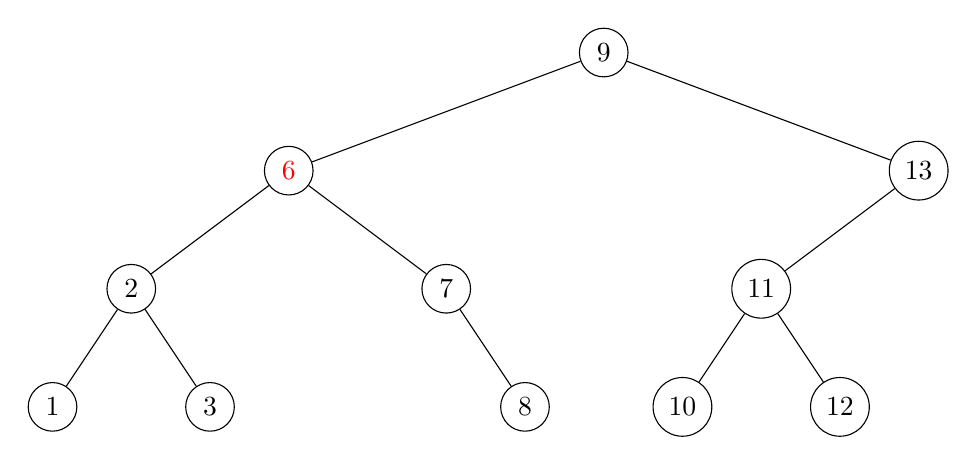
\begin{tikzpicture}[
            level distance=1.5cm,
            level 1/.style={sibling distance=8cm},
            level 2/.style={sibling distance=4cm},
            level 3/.style={sibling distance=2cm}
        ]
        \node[circle,draw] {9}
        child {
                node[circle,draw] {\textcolor{red}{6}}
                child {
                        node[circle,draw] {2}
                        child {node[circle,draw] {1}}
                        child {node[circle,draw] {3}}
                    }
                child {
                        node[circle,draw] {7}
                        child[missing] {}
                        child {node[circle,draw] {8}}
                    }
            }
        child {
                node[circle,draw] {13}
                child {
                        node[circle,draw] {11}
                        child {node[circle,draw] {10}}
                        child {node[circle,draw] {12}}
                    }
                child[missing] {}
            };
    \end{tikzpicture}
\end{figure}

\subsection{红黑树删除结点}

红黑树的删除操作要比插入操作复杂得多。

\subsubsection{第一步}

如果待删除结点有两个非空的孩子结点,转化成待删除结点只有一个孩子(或没有孩子)的情况。 \\

例如删除结点8:

\begin{figure}[H]
    \centering
    \begin{tikzpicture}[font=\sffamily, very thick,
            level distance=1.5cm,
            level 1/.style={sibling distance=2cm},
            level 2/.style={sibling distance=1cm},
            level 3/.style={sibling distance=1cm}
        ]
        \node [blackVertex] (r){8}
        child {
                node [redVertex] {6}
                child {node[rectangle,draw] {1}}
                child {node[rectangle,draw] {2}}
            }
        child {
                node [redVertex] {11}
                child {
                        node [blackVertex] {10}
                        child {node [nil] {NIL}}
                        child {node[rectangle,draw] {3}}
                    }
                child {node[rectangle,draw] {4}}
            };
    \end{tikzpicture}
\end{figure}

因为结点8有两个孩子,可以选择仅大于8的结点10复制到8的位置,结点颜色变成待删除结点的颜色。

\begin{figure}[H]
    \centering
    \begin{tikzpicture}[font=\sffamily, very thick,
            level distance=1.5cm,
            level 1/.style={sibling distance=2cm},
            level 2/.style={sibling distance=1cm},
            level 3/.style={sibling distance=1cm}
        ]
        \node [blackVertex] (r){10}
        child {
                node [redVertex] {6}
                child {node[rectangle,draw] {1}}
                child {node[rectangle,draw] {2}}
            }
        child {
                node [redVertex] {11}
                child {
                        node [blackVertex] {10}
                        child {node [nil] {NIL}}
                        child {node[rectangle,draw] {3}}
                    }
                child {node[rectangle,draw] {4}}
            };
    \end{tikzpicture}
\end{figure}

结点10能成为仅大于8的结点,必定没有左孩子结点,所以问题转换成了待删除结点只有一个右孩子(或者没有孩子)的情况。

\subsubsection{第二步}

根据待删除结点和其唯一子结点的颜色,分情况处理。 \\

\textbf{情况1:}自身是红色,子结点是黑色。直接按照二叉查找树的删除操作,删除结点1即可。

\begin{figure}[H]
    \centering
    \begin{tikzpicture}[font=\sffamily, very thick,
            level distance=1.5cm,
            level 1/.style={sibling distance=2cm},
            level 2/.style={sibling distance=1cm}
        ]
        \node [redVertex] (r){1}
        child {node [nil] {NIL}}
        child {
                node [blackVertex] {2}
                child {node[rectangle,draw] {1}}
                child {node[rectangle,draw] {2}}
            };
    \end{tikzpicture}
\end{figure}

\begin{figure}[H]
    \centering
    \begin{tikzpicture}[font=\sffamily, very thick,
            level distance=1.5cm,
            level 1/.style={sibling distance=2cm},
            level 2/.style={sibling distance=1cm}
        ]
        \node [blackVertex] (r){2}
        child {node[rectangle,draw] {1}}
        child {node[rectangle,draw] {2}};
    \end{tikzpicture}
\end{figure}

\textbf{情况2:}自身是黑色,子结点是红色。按照二叉查找树的删除操作,删除结点1。此时这条路径凭空少了一个黑色结点,因此需要将结点2变成黑色即可。

\begin{figure}[H]
    \centering
    \begin{tikzpicture}[font=\sffamily, very thick,
            level distance=1.5cm,
            level 1/.style={sibling distance=2cm},
            level 2/.style={sibling distance=1cm}
        ]
        \node [blackVertex] (r){1}
        child {node [nil] {NIL}}
        child {
                node [redVertex] {2}
                child {node[rectangle,draw] {1}}
                child {node[rectangle,draw] {2}}
            };
    \end{tikzpicture}
\end{figure}

\begin{figure}[H]
    \centering
    \begin{tikzpicture}[font=\sffamily, very thick,
            level distance=1.5cm,
            level 1/.style={sibling distance=2cm},
            level 2/.style={sibling distance=1cm}
        ]
        \node [redVertex] (r){2}
        child {node[rectangle,draw] {1}}
        child {node[rectangle,draw] {2}};
    \end{tikzpicture}
\end{figure}

\textbf{情况3:}自身是黑色,子结点也是黑色,或者子结点是空叶子结点。这种情况最为复杂,涉及到很多变化。首先还是按照二叉查找树的删除操作,删除结点1。此时这条路径凭空少了一个黑色结点,而且并不能改变结点2的颜色来解决问题。这时需要进入第三步,专门解决父子双黑的情况。

\begin{figure}[H]
    \centering
    \begin{tikzpicture}[font=\sffamily, very thick,
            level distance=1.5cm,
            level 1/.style={sibling distance=2cm},
            level 2/.style={sibling distance=1cm}
        ]
        \node [blackVertex] (r){1}
        child {node [nil] {NIL}}
        child {
                node [blackVertex] {2}
                child {node[rectangle,draw] {1}}
                child {node[rectangle,draw] {2}}
            };
    \end{tikzpicture}
\end{figure}

\subsubsection{第三步}

遇到双黑结点,在子结点顶替父结点后,可分为6种情况处理。 \\

\textbf{情况1:}结点2是红黑树的根。此时所有路径都减少了一个黑色结点,并未打破规则,无需调整。

\begin{figure}[H]
    \centering
    \begin{tikzpicture}[font=\sffamily, very thick,
            level distance=1.5cm,
            level 1/.style={sibling distance=2cm},
            level 2/.style={sibling distance=1cm}
        ]
        \node [blackVertex] (r){2}
        child {node[rectangle,draw] {1}}
        child {node[rectangle,draw] {2}};
    \end{tikzpicture}
\end{figure}

\textbf{情况2:}结点2的父亲、兄弟和侄子结点都是黑色。

\begin{figure}[H]
    \centering
    \begin{tikzpicture}[font=\sffamily, very thick,
            level distance=1.5cm,
            level 1/.style={sibling distance=4cm},
            level 2/.style={sibling distance=2cm},
            level 3/.style={sibling distance=1cm},
        ]
        \node [blackVertex] (r){A}
        child {
                node [blackVertex] {2}
                child {node[rectangle,draw] {1}}
                child {node[rectangle,draw] {2}}
            }
        child {
                node [blackVertex] {B}
                child {
                        node [blackVertex] {C}
                        child {node[rectangle,draw] {3}}
                        child {node[rectangle,draw] {4}}
                    }
                child {
                        node [blackVertex] {D}
                        child {node[rectangle,draw] {5}}
                        child {node[rectangle,draw] {6}}
                    }
            };
    \end{tikzpicture}
\end{figure}

直接把结点2的兄弟结点变为红色。这样结点B所在路径少了一个黑色结点,两边扯平了。

\begin{figure}[H]
    \centering
    \begin{tikzpicture}[font=\sffamily, very thick,
            level distance=1.5cm,
            level 1/.style={sibling distance=4cm},
            level 2/.style={sibling distance=2cm},
            level 3/.style={sibling distance=1cm},
        ]
        \node [blackVertex] (r){A}
        child {
                node [blackVertex] {2}
                child {node[rectangle,draw] {1}}
                child {node[rectangle,draw] {2}}
            }
        child {
                node [redVertex] {B}
                child {
                        node [blackVertex] {C}
                        child {node[rectangle,draw] {3}}
                        child {node[rectangle,draw] {4}}
                    }
                child {
                        node [blackVertex] {D}
                        child {node[rectangle,draw] {5}}
                        child {node[rectangle,draw] {6}}
                    }
            };
    \end{tikzpicture}
\end{figure}